\documentclass[11pt,a4paper]{article}
\usepackage[margin=2.2cm]{geometry}
\usepackage{amsmath,amssymb}
\usepackage{siunitx}
\usepackage{booktabs}
\usepackage{xcolor}
\usepackage{microtype}
\usepackage{enumitem}
\usepackage{tcolorbox}
\usepackage{graphicx}
\definecolor{ink}{HTML}{14231B}\definecolor{accent}{HTML}{0F3D2A}
\tcbuselibrary{skins}
\newtcolorbox{key}{colback=accent!6,colframe=accent,boxrule=0.6pt,arc=2pt,left=6pt,right=6pt,top=4pt,bottom=4pt}
\sisetup{per-mode=symbol,group-separator={\,}}
\setlength{\parindent}{0pt}\setlength{\parskip}{6pt}
\renewcommand{\arraystretch}{1.25}

\title{\textbf{Slide 11: the listener}\\\large WAKE\_N and BIG\_N watch the signal without gating it}
\author{ADS7057 test board v3 \quad ---\quad study notes}\date{}
\begin{document}\maketitle\vspace{-1.2em}
\section{The idea}
The listener is a small second circuit that reads SIG\_IN, the same signal the chain sees. It never switches the capture chain: the chain stays on and the FPGA has the waveform and the listener decisions side by side. Two open-drain lines go to the PMOD: WAKE\_N (medium burst, PMOD pin 10) and BIG\_N (large burst, pin 7). Both are active low.

\section{The circuit}
\begin{center}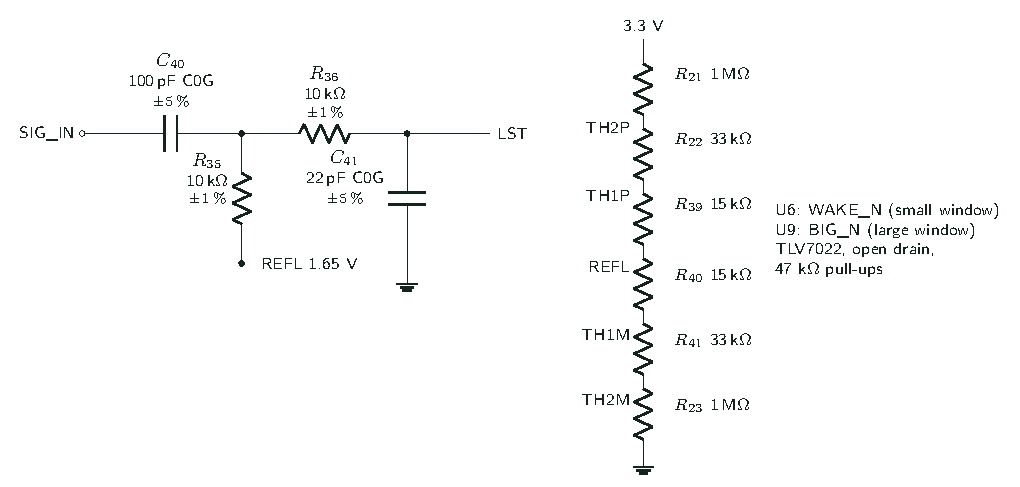
\includegraphics[width=0.98\textwidth]{s11_circuit.pdf}\end{center}

\section{The filter}
C40/R35 is a high-pass with its corner at $1/(2\pi\cdot10\,\text{k}\Omega\cdot100\,\text{pF})=\SI{159}{kHz}$. R36/C41 is a low-pass at $1/(2\pi\cdot10\,\text{k}\Omega\cdot22\,\text{pF})=\SI{723}{kHz}$. R35 returns to REFL, so the output rests at 1.65 V. The second stage loads the first, so the exact gain from the two node equations (not the product of two corners) is
\begin{center}\begin{tabular}{rrrrr}\toprule f & \SI{10}{kHz} & \SI{100}{kHz} & \SI{250}{kHz} & \SI{1}{MHz}\\\midrule
$|H|$ & 0.063 & 0.489 & 0.681 & 0.529\\ dB & $-24.1$ & $-6.2$ & $-3.3$ & $-5.5\,$\\\bottomrule\end{tabular}\end{center}
ngspice on the as-built netlist gives $-3.34$ dB at \SI{250}{kHz} and $-24.06$ dB at \SI{10}{kHz}, the same numbers. The netlist simulation found that the first version of this filter loaded its first stage too much. R36 and C41 were changed to $10\,$k$\Omega$ and \SI{22}{pF} to fix it.

\section{The thresholds}
One chain of resistors from 3.3 V to ground makes all four thresholds: R21 $1\,$M, R22 $33\,$k, R39 $15\,$k, \textbf{REFL}, R40 $15\,$k, R41 $33\,$k, R23 $1\,$M. Total $2.096\,$M$\Omega$, so
\[
I=\frac{3.3}{2.096\,\text{M}\Omega}=\SI{1.574}{\micro A},\qquad V_\text{REFL}=3.3\cdot\frac{1.048}{2.096}=\SI{1.65}{V}.
\]
\[
V_\text{TH1}-V_\text{REFL}=I\cdot15\,\text{k}\Omega=\SI{23.6}{mV},\qquad
V_\text{TH2}-V_\text{REFL}=I\cdot48\,\text{k}\Omega=\SI{75.6}{mV}.
\]
Each comparator pair (U6 for WAKE\_N, U9 for BIG\_N) compares LST with a node above and a node below REFL, so either polarity trips it. Divide by the filter gain 0.681 to refer the thresholds to SIG\_IN:
\[
\text{WAKE\_N: }\frac{23.6}{0.681}=\SI{35}{mV},\qquad \text{BIG\_N: }\frac{75.6}{0.681}=\SI{111}{mV}.
\]
The 47 k$\Omega$ pull-ups (R24, R42) make the lines open drain: the TLV7022 can only pull low. Response time about \SI{260}{ns}, input offset up to $\pm8$ mV and hysteresis about 7 mV, so each threshold is good to about $\pm12$ mV at SIG\_IN.

\section{Against real data}
\begin{center}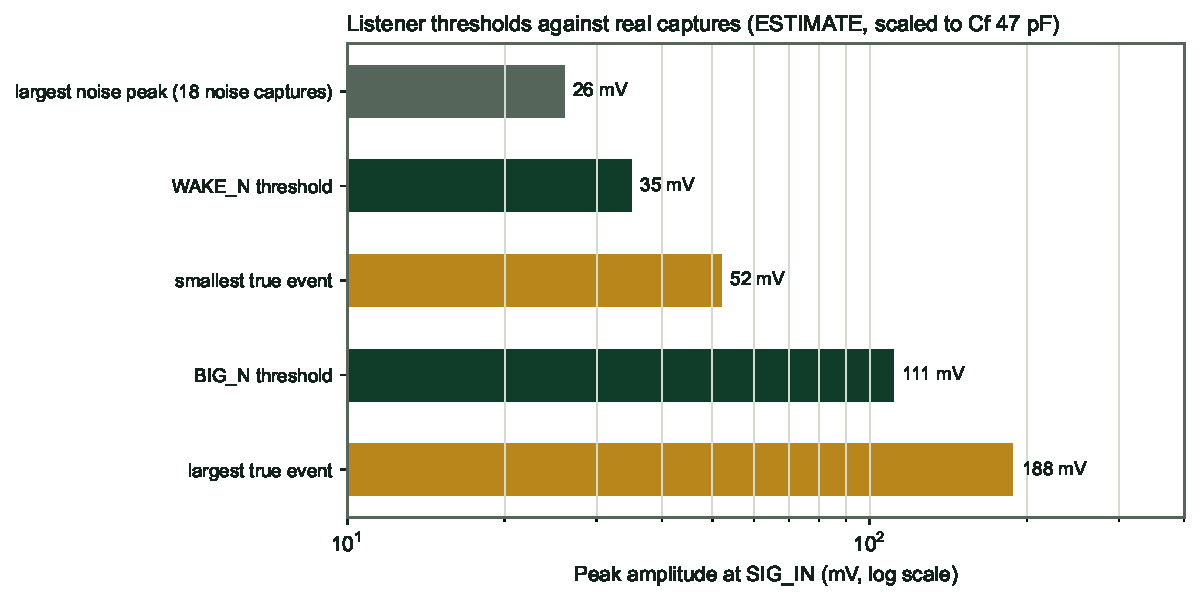
\includegraphics[width=0.85\textwidth]{s11_graph.pdf}\end{center}
On 25 recorded captures (scaled to $C_f=\SI{47}{pF}$, an estimate) the noise after the \SI{100}{kHz} high-pass is \SI{4.0}{mV} rms (worst \SI{9.2}{mV}). The largest noise peak of the 18 noise captures is \SI{26}{mV}, under the \SI{35}{mV} WAKE\_N threshold, a margin of only $1.3\times$. The 7 real events peak at 52 to \SI{188}{mV}, all above it.

\begin{key}
The margin on noise is thin, and the thresholds move with the head. With the OPA314 head ($C_f=\SI{220}{pF}$) volts per pC fall by 4.7 and the ladder must change. Bench test: \SI{250}{kHz} ten-cycle burst; WAKE\_N must fall near \SI{35}{mV} and BIG\_N near \SI{111}{mV} at SIG\_IN.
\end{key}
\end{document}
